\chapter{\jnif{}: \java{} Native Instrumentation}
\label{ap:jnif}

This appendix presents \jnif{}, our library to instrument \java{} applications in native code using \cc{}/\cpp{}.
Although the material presented here is not directly related to this thesis, we have used \jnif{} in several experiments during the development of both Chapters~\ref{cha:unsafe} and~\ref{cha:casts}.
The original article have been published in~\cite{mastrangeloJNIFJavaNative2014}.
Moreover, the source code of \jnif{} can be found online.%
\urlnote{https://gitlab.com/acuarica/jnif}

\section{Introduction}\label{sec:jnif-introduction}

Program analysis tools are important in software engineering tasks 
such as comprehension, verification and validation, profiling, debugging, and optimization.
They can be broadly categorized either as static or dynamic,
based on the input that they take.
Static analysis tools carry out their task using as input only a program
in a given representation, \eg{}, source code, abstract syntax tree,
bytecode, or binary code.
In contrast, dynamic analysis tools observe the program being analyzed 
by collecting runtime information.
Many dynamic analysis tools rely on instrumentation to achieve their goals.

In the context of the JVM, 
static analysis and instrumentation for dynamic analysis often happens on the level of Java bytecode.
Analysis tools thus need to decode and analyze---and in the case of instrumentation also edit and encode---Java bytecode.
Given the relative complexity of the Java class file format,
a diverse set of libraries (see Section~\ref{sec:jnif-relatedwork}) has been created for this purpose.
All those libraries are implemented in Java.

Instrumentation at bytecode level can be done in two ways:
using a \java{} instrumentation agent or using a native \jvmti{} agent.%
\footnote{\url{http://docs.oracle.com/javase/7/docs/technotes/guides/jvmti/index.html}}
A Java instrumentation agent is written in Java and runs in the same JVM as the application.
This leads to two main problems: poor isolation and poor coverage.
It provides \emph{poor isolation} because to instrument the VM, 
the agent's classes must be loaded in the same VM,
and this can lead to perturbation in the VM.
It provides \emph{poor coverage} because 
an instrumentation agent (implemented in Java) will require some runtime library classes to be loaded before it can start instrumenting,
and those runtime classes thus cannot be instrumented at load time. 

A native \jvmti{} agent can instrument every class that the VM loads, including runtime classes. 
The main issue when using \jvmti{} is that instrumentation must be done in a native language, usually C or C++. 
Using C/C++ as the instrumentation language can be problematic, 
because of the lack of a C/C++ library for Java bytecode rewriting. 
Therefore developers have been using an extra JVM as an ``instrumentation server''
in which they could use Java-based bytecode rewriting libraries.
The C/C++ \jvmti{} agent thus only has to send code to the server,
and no native bytecode rewriting library is needed.
However, this approach has a drawback: it requires an additional \jvm{}, 
and it causes IPC traffic between the observed JVM and the instrumentation server.

We created \jnif{} to overcome this problem. 
To the best of our knowledge, \jnif{} is the first native Java bytecode rewriting library.
\jnif{} is a C++ library for decoding, analyzing, editing, and encoding Java bytecode.
The main benefit of \jnif{} is that it can be plugged into a \jvmti{} agent 
for instrumenting all classes in a JVM transparently, i.e., 
without connecting to another \jvm{} and without perturbing the observed \jvm{}.

Starting with \java{} 6, class files can include stack maps to
simplify bytecode verification for the \jvm{}.
\java{} 7 made those stack maps mandatory.
Thus, unless one wants to disable the \jvm{}'s verifier,
code rewriting tools need to also generate stack maps.
Stack maps contain, for each basic block,
type information for each local variable and operand stack slot.
To generate stack maps, a bytecode rewriting tool needs to perform a static analysis.
Due to the fact that bytecode does not contain type declarations of variable slots and local variables,
these types have to be inferred using an intra-procedural data flow analysis.
For reference types, 
computing the least upper bound of two types in a join point of a control flow graph 
even requires access to the class hierarchy of the program.
Thus, the seemingly innocuous requirement for stack maps
significantly complicates the creation of a bytecode rewriting library.
\jnif{} solves these issues, also thanks to the fact that it can be
used in-process in a \jvmti{} agent,
and thus can determine the necessary subtyping relationships 
by requesting the bytes of arbitrary classes loaded or loadable at any given point in time.
This works for classes loaded via user-defined class loaders as well as
for classes generated dynamically on-the-fly.

Overall, the main contributions of this paper are:

\begin{itemize}
	\item We present \jnif{}, a C++ library for decoding, analyzing, editing, and encoding Java class files.
	\item \jnif{} includes a data-flow analysis for stack map generation, 
	      a complication necessary for any library that provides editing and encoding support for modern \jvm{}s with split-time verification.
	\item We evaluate \jnif{} by comparing its performance against the most prevalent Java bytecode rewriting library, ASM.
\end{itemize}

The rest of this chapter is organized as follows:
Section~\ref{sec:jnif-relatedwork} presents related work.
In Section~\ref{sec:jnif-usage} we show how to use the \jnif{} API.
Section~\ref{sec:jnif-implementation} describes the design of \jnif{}.
Section~\ref{sec:jnif-test} explains how we validated \jnif{}.
Section~\ref{sec:jnif-evaluation} evaluates \jnif{}'s performance against the mainstream bytecode manipulator, ASM.
Section~\ref{sec:jnif-limitations} discusses limitations, and 
Section~\ref{sec:jnif-conclusions} concludes.
\section{Related Work}\label{sec:jnif-relatedwork}

We now discuss low-level \java{} bytecode rewriting libraries,
JVM hooks for dynamic bytecode rewriting,
high-level dynamic bytecode rewriting frameworks,
and how they relate to JNIF.
 
\subsection*{Low-level rewriting libraries.}

JNIF certainly is not the first Java bytecode analysis and instrumentation framework.
The probably earliest is BCEL\footnote{\url{http://commons.apache.org/bcel/}},
a well-designed Java library with a tree-based API.
The probably most prevalent is ASM\footnote{\url{http://asm.ow2.org/}}~\citep{brunetonASMCodeManipulation2002,kuleshovUsingASMFramework2007},
which aims to be more efficient, especially due to the addition of a visitor-based streaming API, 
but which has a somewhat less encapsulated design.
SOOT\footnote{\url{http://www.sable.mcgill.ca/soot/}}~\citep{vallee-raiSootJavaBytecode1999}
is a Java bytecode optimization framework supporting whole-program analysis
with four different intermediate representations:
Baf, which is simple to manipulate,
Jimple, which is easy to optimize, 
Shimple, an SSA-based variant of Jimple, and
Grimp, focused on decompilation. 
%
WALA\footnote{\url{http://wala.sourceforge.net/}} is a framework for static analysis, 
which also includes SHRIKE\footnote{\url{http://wala.sourceforge.net/wiki/index.php/Shrike_technical_overview}}, 
a library for instrumenting bytecode using a patch-based approach.
%
Unlike the above libraries, 
Javassist\footnote{\url{http://www.javassist.org/}}~\cite{chibaEasytoUseToolkitEfficient2003}
provides an API for editing class files like they were Java source code,
thereby enabling developers who do not understand bytecode to instrument class files.

\subsection*{Dynamic instrumentation hooks.}

The most limited way for dynamically rewriting \java{} classes at runtime
is the use of a custom class loader.
This requires modifications to the application,
so that it uses that class loader.
This can be problematic for applications---especially for large programs
based on powerful frameworks---that already use their own class loaders.
This limitation can be circumvented by using dynamic instrumentation
hooks provided by the JVM~\cite{lindholmJavaVirtualMachine}.
Java provides two such hooks: Java agents and JVMTI.
Java agents%
\footnote{\url{http://docs.oracle.com/javase/7/docs/api/java/lang/instrument/package-summary.html}} 
are supported via the \texttt{-javaagent} JVM command line argument.
They are implemented in \java{} and use the \code{java.lang.instrument} package to interact with the JVM.
This allows them to get notified when classes are about to get loaded,
and it allows them to modify the class bytecode.
They can also modify and reload already loaded classes,
however the kinds of transformations allowed with class reloading are severely limited.
JVMTI (the \emph{Java Virtual Machine Tool Interface}) is a native API into the JVM that, 
amongst many other things, provides hooks that allow the
rewriting of bytecode.
The advantage of JVMTI over Java agents is that JVMTI allows the instrumentation of \emph{all} Java classes, including the entire runtime library.
Java also provides JDI%
\footnote{\url{https://docs.oracle.com/javase/7/docs/jdk/api/jpda/jdi/}}
(the \emph{Java Debug Interface}), 
a high-level interface on top of JVMTI to control a running application in a remote JVM.

\subsection*{High-level dynamic analysis frameworks.}

We now discuss dynamic analysis frameworks that are built on top of the previously mentioned rewriting libraries
and use the above instrumentation hooks.
These frameworks do not allow arbitrary code transformations 
and they shield the developer from the necessary instrumentation effort.
%
Sofya\footnote{\url{http://sofya.unl.edu}}~\cite{kinneerSofyaSupportingRapid2007} 
is a dynamic analysis framework that runs the analysis in a separate JVM from the observed application.
It provides analysis developers with a set of observable events, to which the analyses can subscribe.
Sofya combines bytecode instrumentation using BCEL with the use of JDI for capturing events.
FERRARI~\cite{binderReengineeringStandardJava2007} is a dynamic bytecode instrumentation framework
that combines static instrumentation of runtime library classes with
dynamic instrumentation of application classes to achieve full coverage.
FERRARI hooks into the JVM using a Java agent.
DiSL~\cite{marekDiSLDomainspecificLanguage2012,marekDiSLExtensibleLanguage2012}
is a domain-specific aspect language for dynamic analysis.
It eliminates the need for static instrumentation from FERRARI
by using a separate JVM for instrumentation.
It uses JVMTI to hook into the JVM and 
forwards loaded classes to an instrumentation server,
where it performs instrumentation using the ASM rewriting library.
Turbo DiSL~\cite{zhengTurboDiSLPartial2012} significantly improves the performance of DiSL 
by partially evaluating analysis code at instrumentation time.
RoadRunner\footnote{\url{http://dept.cs.williams.edu/~freund/rr/}}~\cite{flanaganRoadRunnerDynamicAnalysis2010}
is a high-level framework for creating dynamic analyses focusing on concurrent programs.
An analysis implemented on top of RoadRunner simply consists of analysis code
in the form of a class that can handle the various event types 
(such as method calls or field accesses) that RoadRunner can track.
RoadRunner uses a custom classloader to be able to rewrite classes at load time,
and it uses ASM for bytecode rewriting.
Btrace\footnote{\url{https://kenai.com/projects/btrace}} is an instrumentation tool
that allows developers to inject probes based on a predefined set of probe types
(such as method entry, or bytecode for a specific source line number).
Btrace uses the Java agent hooks and builds on top of ASM for instrumentation.
Chord\footnote{\url{http://pag.gatech.edu/chord/}}~\cite{naik11} is a static analysis framework based on Datalog.
It uses joeq\footnote{\url{http://joeq.sourceforge.net}} to decode classes and 
convert bytecode into a three-address quadcode internal representation for static analysis.
Chord also supports dynamic analysis, 
for which it instruments programs using Javassist.

\subsection*{How JNIF differs.}

Similar to BCEL, JNIF is a low-level library that uses a clean object model to represent java class files.
However, unlike all the libraries described above,
JNIF is not implemented in Java, but in C++.
This allows JNIF to be used directly inside a JVMTI agent. 
Java-based libraries do not allow dynamic instrumentation in this way:
they either are limited to Java agents (which only provide limited coverage),
or they require out-of-process instrumentation inside a second JVM (a so-called instrumentation server),
and inter-process communication between the JVMTI agent and the instrumentation server.

JNIF simplifies the development and deployment of full-coverage dynamic analysis tools,
because one does not need to run an instrumentation server in a separate JVM process.
The fact that this is essential is demonstrated by the HPROF\footnote{\url{http://docs.oracle.com/javase/7/docs/technotes/samples/hprof.html}} profiling agent coming with the JVM.
HPROF does not use Java libraries for rewriting bytecode,
but implements (a limited form of) class file instrumentation as native code inside a JVMTI agent.

The high-level frameworks described above all abstract away from the underlying instrumentation approach.
Thus, they could make use of JNIF to provide their users with full-coverage 
while eliminating the need for a separate instrumentation server.

%Low overhead agent. 
%Modular parser, you pay what you need. 
%Full power of templates for better performance.

%\textbf{Supporting Class File Verification.}
%Java byte code verification~\cite{Leroy:2003:JBV:872715.872719}, 
%its abstract: "Bytecode verification is a crucial security component for Java applets, 
%on the Web and on embedded devices such as smart cards. 
%This paper reviews the various bytecode verification algorithms that have been proposed, 
%recasts them in a common framework of dataflow analysis, and surveys the use of proof assistants to specify bytecode verification and prove its correctness."

\section{Using \jnif{}}\label{sec:jnif-usage}

This section shows common use cases of the \jnif{} library, 
such as writing instrumentation code and analyzing class files, 
thus giving an overview of the library. 
Its components are explained in more detail in Section~\ref{sec:jnif-implementation}.
\jnif{} can be used both in stand-alone tools or
embedded inside a \jvmti{} agent.
The complete \api{} documentation and more extensive examples are available online%
\footnote{\url{http://acuarica.gitlab.io/jnif/}}.
We present the examples in an incremental fashion,
adding complexity in each example.
In order to be able to work with class files, they must me parsed. 
Given a buffer with a class file and its length,
Listing~\ref{usage-parse} shows how to parse it.

\begin{listing}
\begin{minted}{cpp}
const char* data = ...;
int len = ...;

jnif::ClassFile cf(data, len);
\end{minted}
\caption{Decoding a class}
\label{usage-parse}
\end{listing}

The class \code{ClassFile} represents a \java{} class file and contains the definition for each method and fields. 
Besides providing access to all members of a class,
\code{ClassFile} also provides access to the constant pool
via methods like \texttt{getUtf8()} and \texttt{addMethodRef()}.

Once a class file is correctly parsed and loaded it can be manipulated using the methods and fields in \code{ClassFile}.
For instance, in order to write back the parsed class file in a new buffer, the write method is used in conjunction with the computeSize method as shown in listing~\ref{usage-write}.

\begin{listing}
\begin{minted}{cpp}
const char* data = ...;
int len = ...;
jnif::ClassFile cf(data, len);
int newlen = cf.computeSize();
u1* newdata = new u1[newlen];
cf.write(newdata, newlen);

// Use newdata and newlen

delete [] newdata;
\end{minted}
\caption{Encoding a class}
\label{usage-write}
\end{listing}

The \code{ClassFile} class has a collection of fields and methods which can be used to discover the members of the class file. 
The listing~\ref{usage-print} prints in the standard output every method's name and descriptor in a class file. 
Note that every jnif class overloads the \verb|operator<<| in order send it to an \code{std::ostream}.

\begin{listing}
\begin{minted}{cpp}
const char* data = ...;
int len = ...;
jnif::ClassFile cf(data, len);
for (jnif::Method* m : cf.methods) {
	cout << "Method: ";
	cout << cf.getUtf8(m->nameIndex);
	cout << cf.getUtf8(m->descIndex);
	cout << endl;
}
\end{minted}
\caption{Traversing all methods in a class}
\label{usage-print}
\end{listing}

To hook every invocation of a constructor, a method named \code{<init>} in \java{} bytecode, 
one can traverse the method list and check whether the current method is an \code{<init>} method. 
Once detected, it is possible to add instrumentation code, like for instance call a static method in a given class. 
Figure~\ref{usage-alloc} shows how to add instruction to the instruction list.

\begin{listing}
\begin{minted}{cpp}
ConstIndex mid = cf.addMethodRef(classIndex, 
  "alloc", "(Ljava/lang/Object;)V");

for (Method* method : cf.methods) {
	if (method->isInit()) {
		InstList& instList = method->instList();

		Inst* p = *instList.begin();
		instList.addZero(OPCODE_aload_0, p);
		instList.addInvoke(OPCODE_invokestatic, mid, p);
	}
}
\end{minted}
\caption{Instrumenting constructor entries}
\label{usage-alloc}
\end{listing}

Another common use case is to instrument every method entry and exit. In order to do so, one can add the instrumentation code at the beginning of the instruction list to detect the method entry. To detect method exit, it is necessary to look for instructions that terminate the current method execution, i.e., xRETURN family and ATHROW as showed in figure~\ref{usage-methodentryexit}.

\begin{listing}
\begin{minted}{cpp}
ConstIndex sid = cf.addMethodRef(proxyClass, "enterMethod",
				"(Ljava/lang/String;Ljava/lang/String;)V");
ConstIndex eid = cf.addMethodRef(proxyClass, "exitMethod",
				"(Ljava/lang/String;Ljava/lang/String;)V");
ConstIndex classNameIdx = cf.addStringFromClass(cf.thisClassIndex);

...

InstList& instList = method->instList();

ConstIndex methodIndex = cf.addString(m->nameIndex);

Inst* p = *instList.begin();

instList.addLdc(OPCODE_ldc_w, classNameIdx, p);
instList.addLdc(OPCODE_ldc_w, methodIndex, p);
instList.addInvoke(OPCODE_invokestatic, sid, p);

for (Inst* inst : instList) {
	if (inst->isExit()) {
		instList.addLdc(OPCODE_ldc_w, classNameIdx, inst);
		instList.addLdc(OPCODE_ldc_w, methodIndex, inst);
		instList.addInvoke(OPCODE_invokestatic, eid, inst);
	}
}
\end{minted}
\caption{Instrumenting \code{<init>} methods}
\label{usage-methodentryexit}
\end{listing}

\section{\jnif{} Design and Implementation}
\label{sec:jnif-implementation}

\jnif{} is written in C++11~\citep{ISO:2012:III}, 
in an object-oriented style similar to \java{}-based class rewriting \api{}s.

\subsection*{Design}

\jnif{} consists of five main modules: model, parser, writer, printer, and analysis.
%
\emph{Model} implements \jnif{}'s intermediate representation.
It is centered around its \code{ClassFile} class. 
It is possible to create and manipulate class files from scratch.
%
\emph{Parser} implements the parsing of class files from a given byte array.
The parser parses a byte array and translates it to the model's IR.
Once a \texttt{ClassFile} is created by the parser,
it can be manipulated with the methods available in the model.
%
\emph{Writer} and \emph{printer} represent two back-ends for the model.
%
\emph{Writer} serializes the entire \texttt{ClassFile} into a byte array ready to be loaded inside a JVM.
%
\emph{Printer} instead serializes the \texttt{ClassFile} into a textual format useful for debugging.
%
Finally, \emph{analysis} implements the static analyses necessary for computing stack maps.


\subsubsection*{JVM-Independence}

\jnif{} is a stand-alone C++ library that can be used outside a JVM.
It does not depend on \jvmti{} or JNI.
However, for the purpose of stack map generation,
it may need to determine the common super class of two classes.
For this it will need to retrieve a class file given the name of an arbitrary class. 
This functionality is provided by a plugin that implements \jnif{}'s \texttt{IClassPath}.
\jnif{} comes with such a plugin that uses JNI in case it is running inside a JVM.


\subsubsection*{Explicit Constant Pool Management}

Unlike some other class rewriting libraries, \jnif{} exposes the constant pool instead of hiding it.
Our reasons for this design decision were two-fold:
(1) We wanted to fully control the structure of the class file, 
and for that it is necessary to expose the constant pool. 
To reduce the additional complexity, we provide a rich set of methods that facilitate constant pool management. 
(2) We wanted to preserve, whenever possible, the original structure of the class file. 
This means that if one parses and then writes a class file, 
the original bytes will be obtained. 
This decreases the perturbation done by the instrumentation and allows for better testing.


\subsubsection*{Memory Management}

Given that \jnif{} is implemented in an unmanaged language,
we have to worry about memory deallocation.
Our API follows a simple ownership model
where all IR objects are owned by their enclosing objects.
This means, that the \texttt{ClassFile} object owns the complete IR of a class.
Our API design enforces this ownership model
by requiring IR objects to be created by their enclosing objects.
For example, to create a \texttt{Method}, 
one has to use the \texttt{ClassFile::addMethod()} factory method
instead of directly allocating a new \texttt{Method} object.


\subsection*{Stack Map Generation}

When encoding a \texttt{ClassFile} into a byte array, \jnif{} needs to generate stack maps.
The necessary static analyses are implemented in the analyzer module.
This module uses data flow analysis and abstract interpretation to determine the types of operand stack slots and local variables.
The analysis module first builds a control flow graph of the method.
The data flow analysis associates to each basic block an input and output stack frame, 
which represents the types of the local variables and operand stack slots at that point in the code.
The input frame represents the type before any instruction in the basic block is executed.
The output frame is computed by abstract interpretation of each instruction in the basic block.
The entry basic block has an empty stack and each entry in its local variable table is set to top.
Then the algorithm starts from the entry block and follows each edge.
If a basic block is reachable from multiple edges, then a merge is involved.

Merging involves finding the least upper bound of multiple incoming types.
While this is trivial for primitive types,
it can require access to the class hierarchy for reference types.
This requirement represents a severe complication for binary rewriting tools:
when rewriting a single class, they may require access to many other classes in the program.
\jnif{} solves this problem by providing the \texttt{IClassPath} interface.
Different \texttt{IClassPath} implementations can provide different ways for getting access to classes.
For example, a static instrumentation tool may use a user-defined class path to find classes,
while a dynamic instrumentation tool may use JNI to request the bytes of a class given that class' name.

%\todo{Problem of finding common super class. 
%How this issue is broken in ASM, 
%because it will cause a lot of class loading and hence static initializer to be run in an order that was not the one assumed by the programmer.}

\subsection*{Running \jnif{} Inside a \jvmti{} Agent}
When using \jnif{} inside a \jvmti{} agent, 
\jnif{} uses an \texttt{IClassPath} implementation
that uses \jni{} to load the bytes of classes
required for least upper bound computations during stack map generation.

\subsubsection*{Avoiding Premature Static Initialization}
Using JNI to load a class (with \texttt{ClassLoader.loadClass()}), however, will call that class' static initializer.
This is a side effect that may change the observable behavior of the program under analysis.
To avoid this, one can request the bytes of the class (with \texttt{ClassLoader.getResourceAsStream())} instead of loading the class.
It can then parse the bytes of the class into its IR to determine that class' supertypes.

\subsubsection*{Avoiding the Loading of the Class Being Instrumented}
If during the instrumentation of a class \code{X} \jnif{} needs to
perform a least upper bound computation involving type \code{X},
then using \code{ClassLoader.loadClass()} to load class \code{X} would
cause an infinite recursion.
The above solution with \code{get\-ResourceAsStream()} also prevents this problem.

\subsubsection*{Avoiding Premature ClassNotFoundException}
If during the instrumentation of a class \texttt{X}
\jnif{} needs to perform a least upper bound computation involving a type \texttt{Y},
and if class \texttt{Y} cannot be found,
then throwing a \texttt{ClassNotFoundException} at that time would be premature
(because without instrumentation, such an exception would only be thrown later).
We solve that problem by assuming a least upper bound of \verb=java.lang.Object= in that case.



%\subsection{Features}
%
%The \jnif{} also provides a convenient way to output dot files from generated control flow graph in order to better understand and analyze complex methods.
%
%Architecture and design picture.?
%
%\subsection{Portability?}
%
%The library uses only C++11 and STL constructions, thus there are no dependencies with any third-party library. Currently the \jnif{} compiles and runs on Linux and MacOS.
%
%
%\begin{lstlisting}[caption=Dots,label=usage-parse2]
%> make dots
%\end{lstlisting}
%
\section{Validation}
\label{sec:jnif-test}

We used a multitude of testing strategies to ensure \jnif{} is working correctly.

The \jnif{} parser and writer makes no extra modification to the class file, 
thus it is an exact representation of the class file. 
This property makes the parser and writer returns the identical same byte stream which can be useful for testing purposes.


\subsection*{Unit Tests}

\jnif{} includes a unit test suite that tests individual features of its various modules.

\subsection*{Integration Tests}

Our integration test suite includes six different \jnif{} clients we run on over 40000 different classes.
Each test reads, analyses, and possibly modifies, prints, or writes classes from the \java{} runtime library (rt.jar),
and all Dacapo benchmarks, \scala{} benchmarks, and the JRuby compiler.

\begin{description}
\item[testPrinter.]
This test parses and prints all classes.
Its main goal is to cover the printing functionality.
It has no explicit assertions.
We consider it passed if it does not throw any exceptions.
\item[testSize.]
This test covers the decoding and encoding modules.
It asserts that the encoded byte array has the same length as the original byte array.
\item[testWriter.]
This is similar to testSize,
but it asserts that the contents of the encoded byte array is identical to the original bytes.
\item[testNopAdderInstrPrinter.]
This also tests the instrumentation functionality,
by injecting NOP instructions and dumping the result.
It passes if it does not throw any exceptions.
\item[testNopAdderInstrSize.]
This is similar to testSize, however it performs NOP injection.
The resulting size must be identical to the original size plus the size of the injected NOP instructions.
\item[testNopAdderInstrWriter.]
This is similar to testNopAdderInstrSize,
but it asserts that the resulting array is identical except for the modified method bytecodes.
\end{description}

The ``size'' and ``writer'' tests work thanks to the fact that 
\jnif{} produces output identical to its input 
as long as classes are not modified and stack maps do not need to be re-generated.


\subsection*{Live Tests}

Our live tests use \jnif{} inside a \jvmti{} dynamic instrumentation agent
to ensure that the output of \jnif{} can successfully be loaded,
verified, and run by a \jvm{}.
In addition to the aspects covered by the unit and integration tests,
the live tests also validate that stack map generation works correctly,
essentially by using the \jvm{}'s verifier to check correctness.
For the live tests, we run a set of microbenchmarks, 
the Dacapo benchmarks, the Scala Benchmarking Project%
\footnote{\url{http://www.benchmarks.scalabench.org/}},
and a microbenchmark using the JRuby compiler,
with the goal of including InvokeDynamic bytecode instructions generated by JRuby.


\subsection*{Assertions and Checks}

The \jnif{} code is sprinkled with calls to \code{Error::assert} 
that check preconditions, postconditions, and invariants.
To provide a developer experience similar to \java{}'s,
all assertion violations print out call stack traces in addition to understandable error messages.

Moreover, \jnif{} checks its inputs (such as class files while parsing, or instrumented code while generating stack maps),
and it calls \code{Error::check} to throw exceptions with stack traces and helpful messages
when checks fail.

\section{Performance Evaluation}\label{sec:jnif-evaluation}

We evaluated the performance of a \jnif{}-based dynamic instrumentation approach 
versus an approach using an ASM-based instrumentation server.

\subsection*{Measurement Contexts}

%\todo{Stecklov?}
%\todo{Yudi's machine?}
%\todo{Luis' Mac?}
We ran our experiments on three different machines:
(1) A machine with two Intel Xeon E5-2620 2~GHz CPUs, 
each with 6 cores and 2 threads per core, 
and 8~GB RAM,
running Debian Linux x86 64 3.10.11-1.
(2) A Dell PowerEdge M620, 2 NUMA node with 64 GB of RAM, 
Intel Xeon E5-2680 2.7~GHz CPU
with 8 cores, 
CPU frequency scaling and Turbo Mode disabled,
running Ubuntu Linux x86 64 3.8.0-38.
For consistent memory access speed, 
we bound our program to a specific NUMA node using \texttt{numactl}.
(3) A MacBook Pro with an Intel Core i7 2.7~GHz CPU 
with 4 cores and 16~GB
running Mac OS X 10.8.2.

%
%For consistent memory access speed, you should add the following before your command,
%which will bind your program in the same NUMA node.
%numactl --cpubind=0 --membind=0
%or
%numactl --cpubind=1 --membind=1




\subsection*{Benchmarks}

We used the Dacapo benchmarks, 
except for tradebeans and tradesoap,
which suffer from a well known issue\footnote{\url{http://sourceforge.net/p/dacapobench/bugs/70/}}.
We also include the Scala benchmarks (except for the subset identical to Dacapo).


%\subsection{Metrics}
%We compare several aspects between the instrumentation made by JNIF and ASM.
%These aspects include time and memory.



\subsection*{Subjects}
We compare \jnif{} to \asm{} for the purpose of performing dynamic instrumentation.
For \jnif{} we built a \jvmti{} agent that directly includes \jnif{} to instrument loaded classes.
For \asm{}, we use a \jvmti{} agent that forwards loaded classes to an instrumentation server
that uses \asm{}'s streaming \api{} (which is faster than \asm{}'s tree API).


\subsection*{Results}

Figure~\ref{fig:instr-time} shows the results of our performance evaluation
in terms of time spent instrumenting classes.
The figure shows the results from our first machine.
The other machines produced results similar to Figure~\ref{fig:instr-time}.
The figure shows box plots summarizing five measurement runs.
It shows one box for JNIF and two boxes for ASM.
The ``ASM Server'' box represents the time as measured on the instrumentation server.
This is equivalent to the time a static instrumentation tool would take.
It excludes the time spent in the JVMTI agent and the time for the IPC between the agent and the server.
The ``ASM Server on Client'' box represents the total time needed for instrumentation, 
as measured in the JVMTI agent,
and thus includes the IPC and JVMTI agent time.

Each chart in the figure consists of five groups of boxes:
``Empty'' is the time when using a JVMTI agent that does not process bytecodes at all.
``Identity'' is for an agent that simply decodes and encodes each class, without any instrumentation, and without recomputing stack maps.
``ComputeFrames'' also includes recomputing stack maps.
``Allocations'' represents a useful dynamic analysis that captures all allocations.
``Nop Padding'' is a different dynamic analysis that injects NOPs after each bytecode instruction. 

The figure shows that frame computation adds significant overhead, on ASM as well as JNIF.
Moreover, it shows that except for dacapo-eclipse, dacapo-jython, and scala-scalatest,
JNIF is faster even than just the ASM Server time.

% \ignore{
% \begin{figure*}[htb]
% \centering
% \vspace{-1cm}
% \includegraphics[width=\textwidth]{../eval-dacapo-chart-instr}

% \vspace{-5mm}
% \includegraphics[width=\textwidth]{../eval-scala-chart-instr}

% \vspace{-5mm}
% \caption{Instrumentation time on DaCapo and Scala benchmarks}
% \label{fig:instr-time}
% \end{figure*}
% }

\begin{figure}[t]
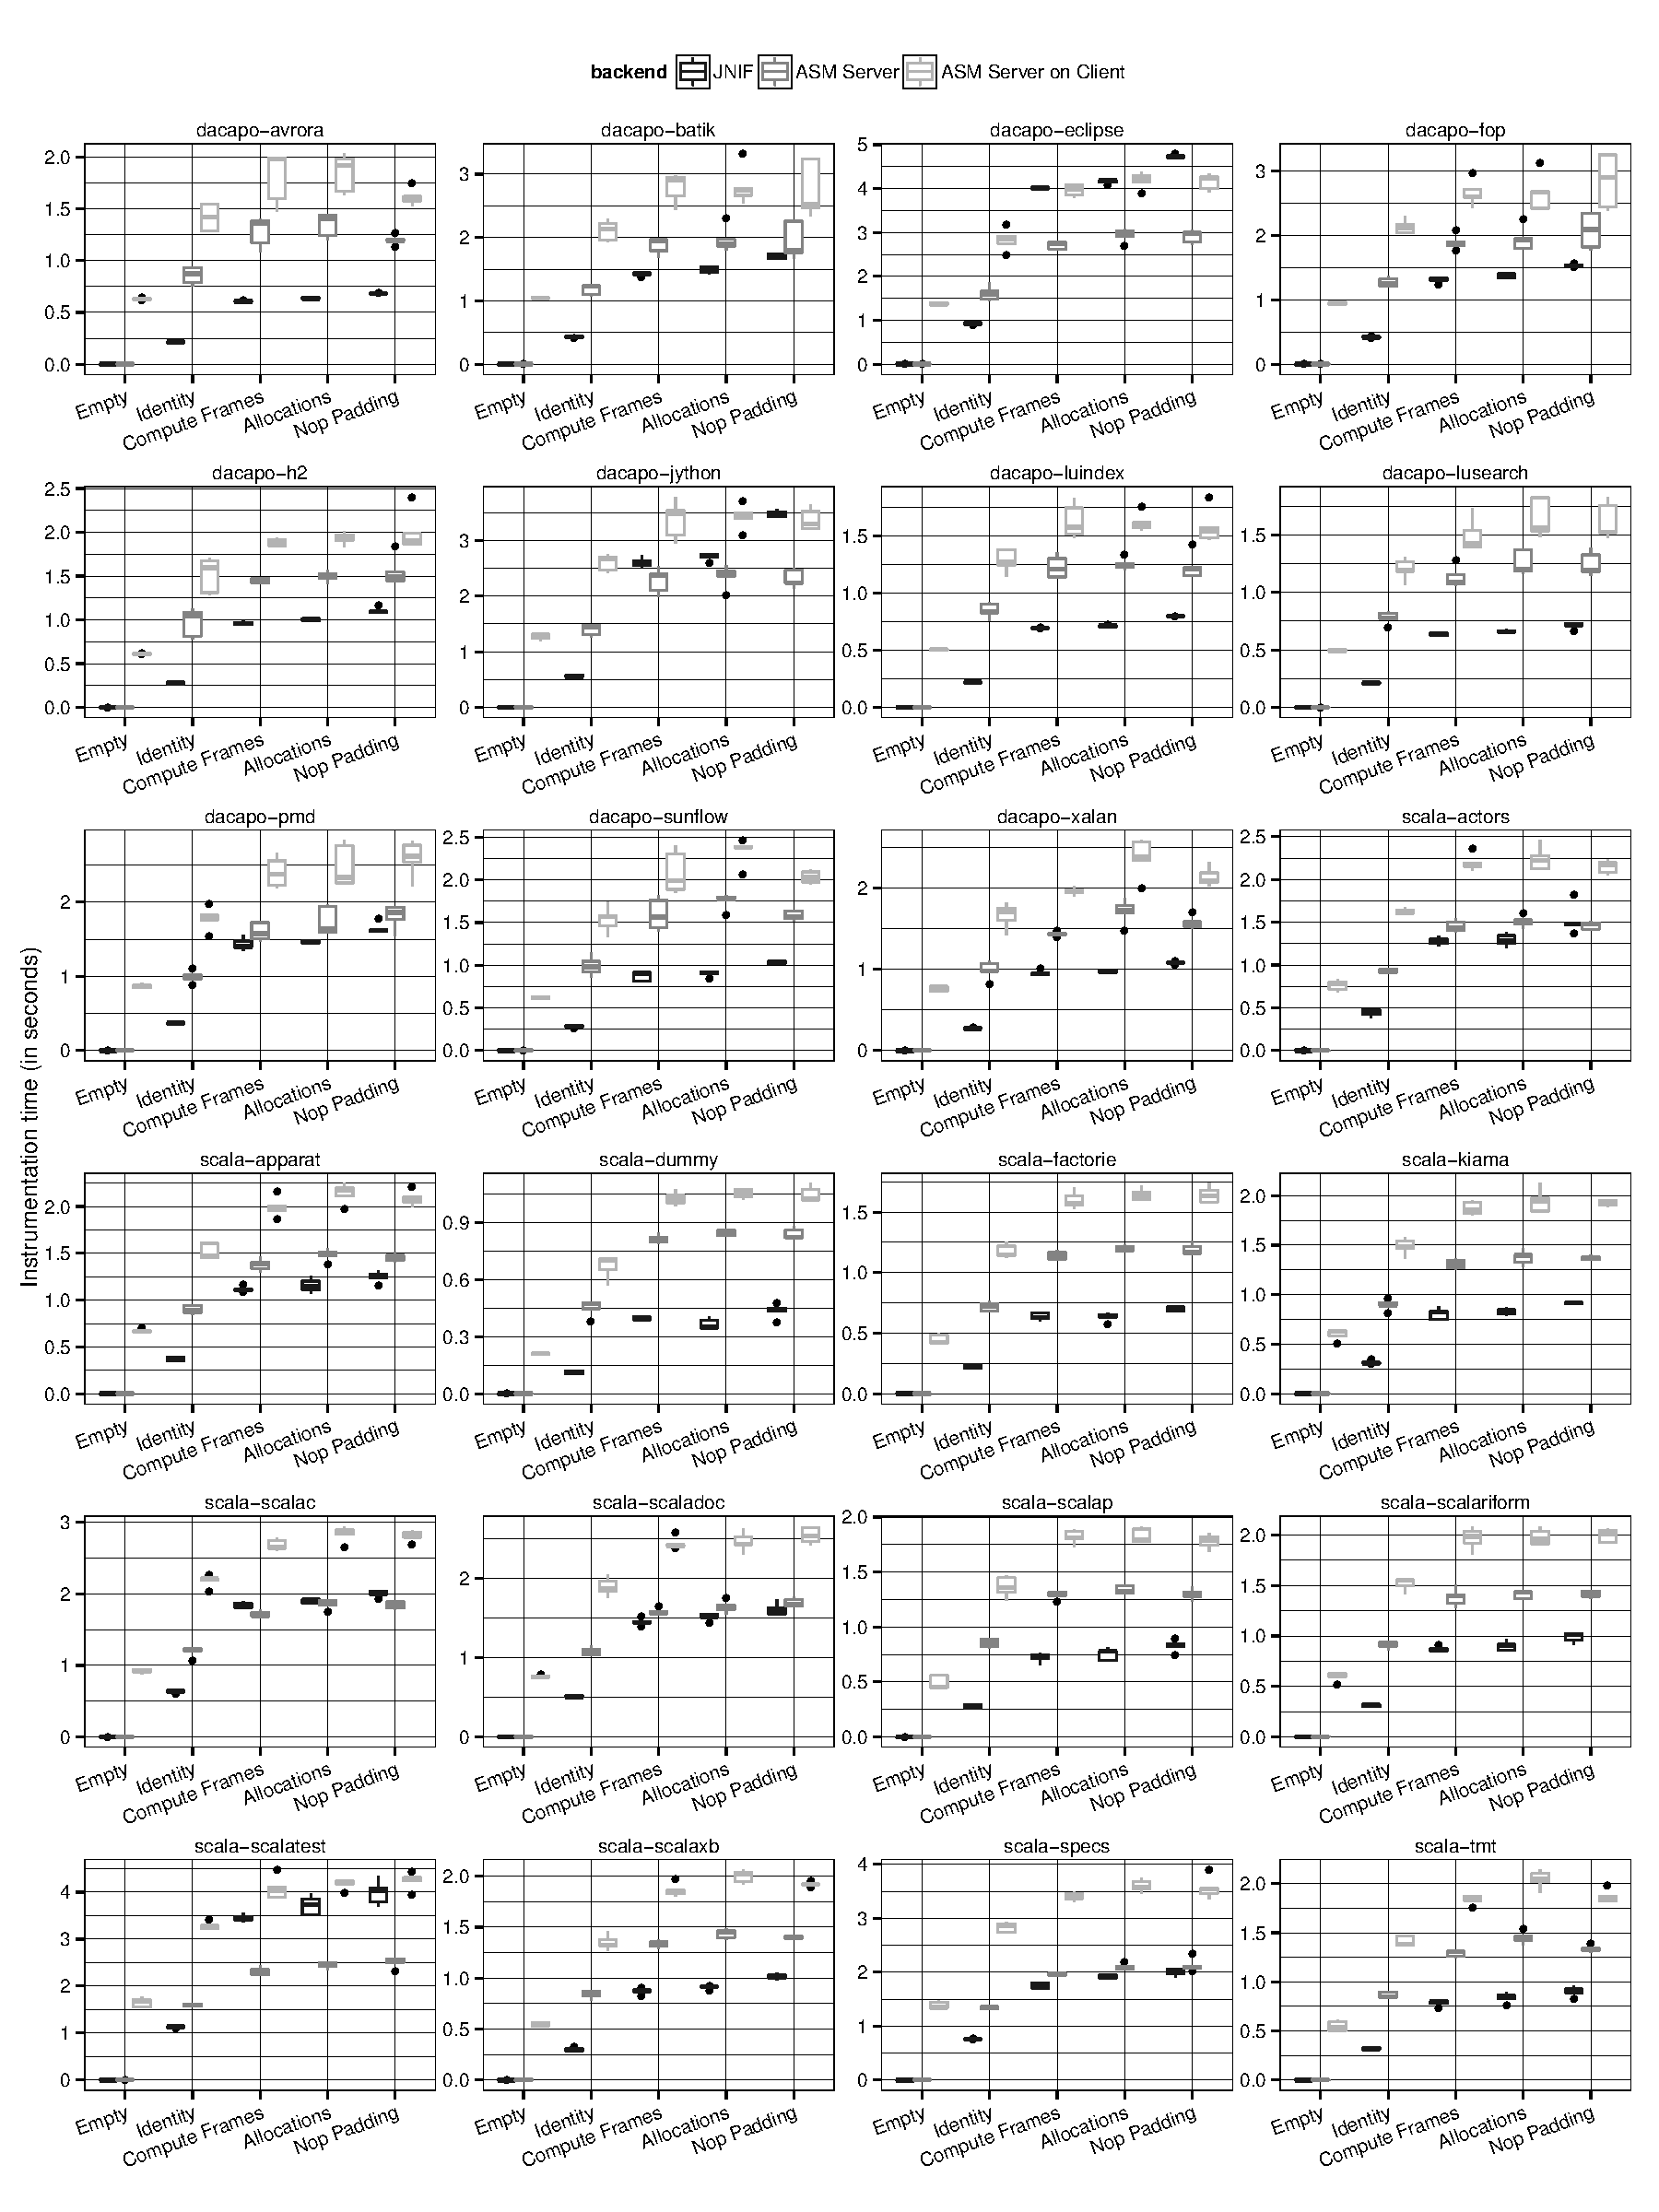
\includegraphics[width=\textwidth]{chapters/jnif/eval-all-chart-instr}
\caption{Instrumentation time on DaCapo and Scala benchmarks}
\label{fig:instr-time}
\end{figure}

%\chart{eval-dacapo-chart-instr}{Instrumentation time on DaCapo}{fig:instr-time-dacapo}
%\chart{eval-scala-chart-instr}{Instrumentation time on Scala and JRuby}{fig:instr-time-scala}

\subsection*{Reproducibility}

To run these evaluations, a Makefile script is provided in the git repository.
These tasks take care of the compilation of the JNIF library and also all java files needed. 
The repository is self-contained, no need to download dacapo benchmarks separately.

\begin{listing}
\begin{minted}[linenos=false]{text}
> make testapp
\end{minted}
\caption{Running testapp}
\label{usage-parse2}
\end{listing}

\begin{listing}
\begin{minted}[linenos=false]{text}
> make testapp
\end{minted}
\caption{Running dacapo}
\label{usage-parse3}
\end{listing}

To run a particular dacapo benchmark with default settings

\begin{listing}
\begin{minted}[linenos=false]{text}
> make dacapo BENCH=avrora
\end{minted}
\caption{Running dacapo}
\label{usage-parse4}
\end{listing}

To run a full evaluation with all dacapo benchmarks in all configuration a task -eval- is provided. You can set how many times run each configuration with the variable times, like

\begin{listing}
\begin{minted}[linenos=false]{text}
> make eval times=5
\end{minted}
\caption{Running full eval five times}
\label{usage-parse5}
\end{listing}

Finally, there is a task to create plots for the evaluation.
This task needs R with the package ggplot2.

\begin{listing}
\begin{minted}[linenos=false]{text}
> make plots
\end{minted}
\caption{Plots}
\label{usage-parse6}
\end{listing}

%1. Stand-alone test-unit:
%In this stage we only test basic functionality of the API such as get the
%right size and the ability to parse and write without correctly without
%any modification and with them. The use of this kind of tests rely on the
%property of the API that if no modification is done to the model the 
%writer is able to recover the original bytes of the class files (except with
%the non-unique property of the stack map tables).
%
%2. Minimal native agent:
%At this stage we prepared several kind of transformations (instrumentation)
%including the identity transformation to test if model/parser/analysis/writer
%can be executed correctly inside a JVM.
%
%3. Dacapo benchmarks:
%As the final tests we run those instrumentations on the Dacapo benchmarks 
%to stress the API. Moreover we use this stage to perform our evaluation.

\section{Limitations}\label{sec:jnif-limitations}

\jnif{} still has some limitations.

\textbf{jsr/ret.} \jnif{} does not support stack map generation for \code{jsr} and \code{ret}.
Class files requiring stack maps do not include \code{jsr}/\code{ret}.
The \code{jsr}/\code{ret} instructions make the control flow graph generation difficult, because a \code{ret} instruction can jump to multiple targets instead of a predefined one.

\textbf{invokedynamic.} \jnif{}'s support for \code{invokedynamic} is not yet fully tested, 
but our initial tests with JRuby have been successful.
Dacapo bach was released in 2009,
before the creation of \java{} 7,
which introduces the \code{invokedynamic} instruction.
Thus it does not contain any benchmark with \code{invokedynamic}.
Instead we use JRuby 1.7 in order to create a self-contained jar file. 
This jar file does not contain any \code{invokedynamic} instruction, 
but it does contain the JRuby compiler, 
that when specified via \code{-Djruby.compile.invokedynamic=true} it will generate class files with \code{invokedynamic}. 
We tested our parser and writer with this settings with successful results.

\textbf{Stack map generation with full coverage.}
When the \jvm{} loads the first few runtime library classes,
and calls the \jvmti{} agent to have those classes instrumented,
it is still too early to use \jni{} for loading classes needed for computing least upper bounds for stack map generation.
For this reason, we do not generate stack maps for runtime library classes.
This no problem, because the \jvm{} does not verify the runtime library classes by default,
and thus it does not need stack maps for those classes.
However, should developers decide to explicitly turn on the verification of runtime library classes
(with \code{-Xverify:all}), the verifier would complain because \jnif{} would not have generated stack maps.

To get full coverage for the instrumentation inside a \jvmti{} agent, 
it is necessary to instrument every class, 
even the whole java class library.
If the instrumentation needs to change or add branch targets, 
the compute frames option must be used, 
but it cannot be used against the class library,
because to compute frames, 
the class hierarchy must be known,
and this imposes a dependency with a classloader which is not yet available.

Luckily, by default the \java{} library classes are not verified,
because they are trusted. 
Thus the instrumentation only needs to compute frames on classes not belonging to the \java{} library.

\section{Conclusions}\label{sec:jnif-conclusions}

Until now,
full-coverage dynamic instrumentation in production \jvm{}s required performing the code rewriting in a separate \jvm{}, 
because of the lack of a native bytecode rewriting framework.
This paper introduces \jnif{}, the first full-coverage in-process dynamic instrumentation framework for Java.
It discusses the key issues of creating such a framework for Java---such as stack-map generation---and
it evaluates the performance of \jnif{} against the most prevalent Java-level framework: ASM.
We find that \jnif{} is faster than using out-of-process ASM in most cases.
We hope that thanks to \jnif{}, and this paper, a broader number of researchers and developers will
be enabled to develop native \jvm{} agents that analyze and rewrite Java bytecode without limitations.
